\chapter{Methods}

\epigraph{``It is not unscientific to make a guess, although many people who are not in science think it is."}{\textit{R. P. Feynman}}


\begin{itemize}
\item Need to preserve spatial information for symbolic front-end
\item Need disentangled latent space for symbolic front-end
\item This may be summarised as needing to be able to deduce the object type and its location solely from the latent space representation
\item Explain degree of freedom here (disentangled filters, or disentangled neurons, or something else?)
\item This is unexplored territory - we decide what the reasonable architecture should be, then evaluate it in the results section
\item As far as we know, this section contains the first considerations of a convolutional variational latent space
\end{itemize}

\label{ch:methods}


%
%
%
%
%
\section{Single Latent Filter}

\begin{itemize}
\item As mentioned, the type and position of an object must be preserved in the latent space
\item This may be achieved by using a single latent filter, with the object type corresponding to the value of the weighted sum of the neuron.
\item Recall that no activation function is used for these layers, and therefore the object type is represented by an unbounded real number
\item Although it's suspected that this may be too much to ask from the network, we still grant it the possibility to surprise us
\end{itemize}

%
%
\subsection{Architecture}
\begin{itemize}
\item The input image is passed through convolutional layers to build increasingly meaningful hidden representations
\item The convolutional mean $\vec{\mu}$ and variance $\vec{\sigma}^2$, both of shape $(1, m, n)$, are sampled using ... cite reparameterisation trick here... (so we may use backpropagation) to give the latent space of shape $(1, m, n)$. 
\item The corresponding deconvolutional layers are applied to reconstruct the original image
\item The proposed architecture is shown in Figure (\ref{fig:latent_image_architecture})
\end{itemize}

\begin{figure}[H]
\centering
\captionsetup{justification=centering}
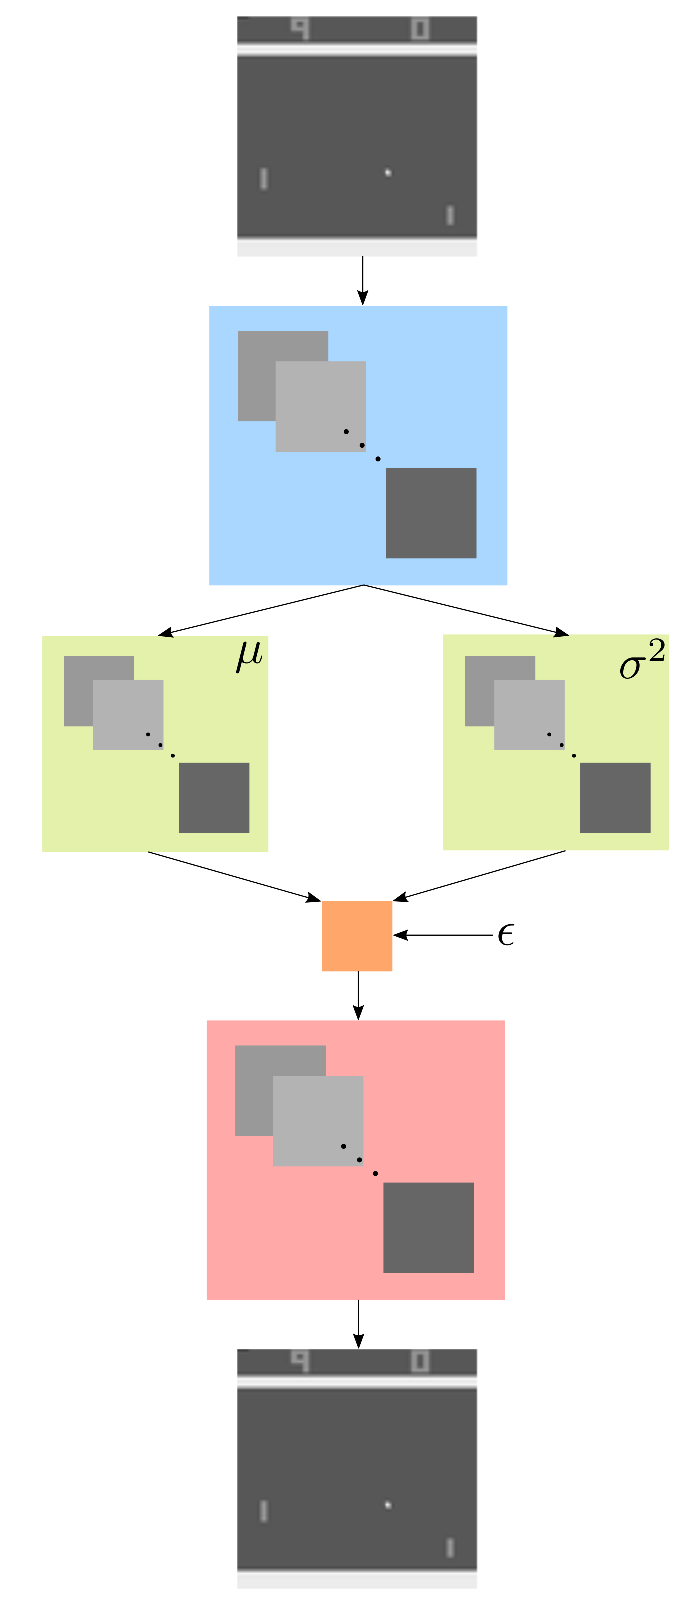
\includegraphics[scale=0.6]{methods/latent_image_architecture.eps}
\caption{The fully-convolutional single latent filter architecture. \textbf{Blue:} An arbitrary amount of convolutional layers. \textbf{Green:} The latent mean $\vec{\mu}$ and variance $\vec{\sigma}^2$, which are both single filters of shape $(1, m, n)$. \textbf{Orange:} A single latent filter of shape $(1, m, n)$ sampled component-wise from $\vec{\mu}$ and $\vec{\sigma}^2$. \textbf{Red:} The corresponding deconvolutional layers.}
\label{fig:latent_image_architecture}
\end{figure}

%
%
\subsection{Derivation}
\begin{itemize}
\item As with the variational autoencoders seen earlier, we have a reconstruction loss term in the loss function
\item Learning the identity function ensures a meaningful lower-dimensional representation is learnt in the latent space
\item However, as we only want values of high magnitude where there are objects, we need to reduce the reundancy in the latent space
\item Therefore we need to decide on the appropriate term in the loss function to reduce redundancy
\item The latent filter of shape $(1, m, n)$ is flattened to a $m \times n$ vector
\item This flattened representation of the single latent filter is used then pressured to be close to an isotropic Gaussian with KL divergence ...equation here...
\item This pressuring reduces redundancy in the latent space as if neighbouring pixels 
\end{itemize}

\begin{figure}[H]
\centering
\captionsetup{justification=centering}
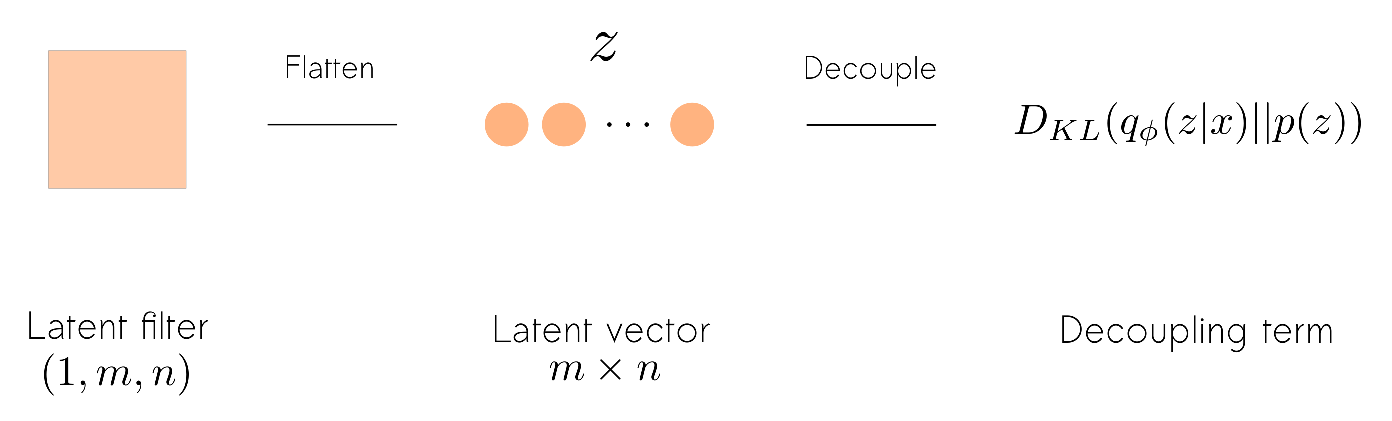
\includegraphics[scale=0.6]{methods/latent_image_flattening_latent_space.eps}
\caption{Caption.}
\label{fig:latent_image_flattening_latent_space}
\end{figure}


%
%
%
%
%
\section{Multiple Latent Filters}
\lipsum[2]

%
%
\subsection{Architecture}
TODO: Finish subsection

\begin{itemize}
\item The architecture is the same as the fully-convolutional single lantent filter architecture, but with one difference in the latent space.
\item The convolutional mean $\vec{\mu}$ and variance $\vec{\sigma}^2$, both of shape $(k, m, n)$, are sampled using ... cite reparameterisation trick here... (so we may use backpropagation) to give the latent space of shape $(k, m, n)$. 
\item The proposed architecture is shown in Figure (\ref{fig:decoupling_indiscriminately_horizontal})
\end{itemize}

\begin{figure}[h!]
\centering
\captionsetup{justification=centering}
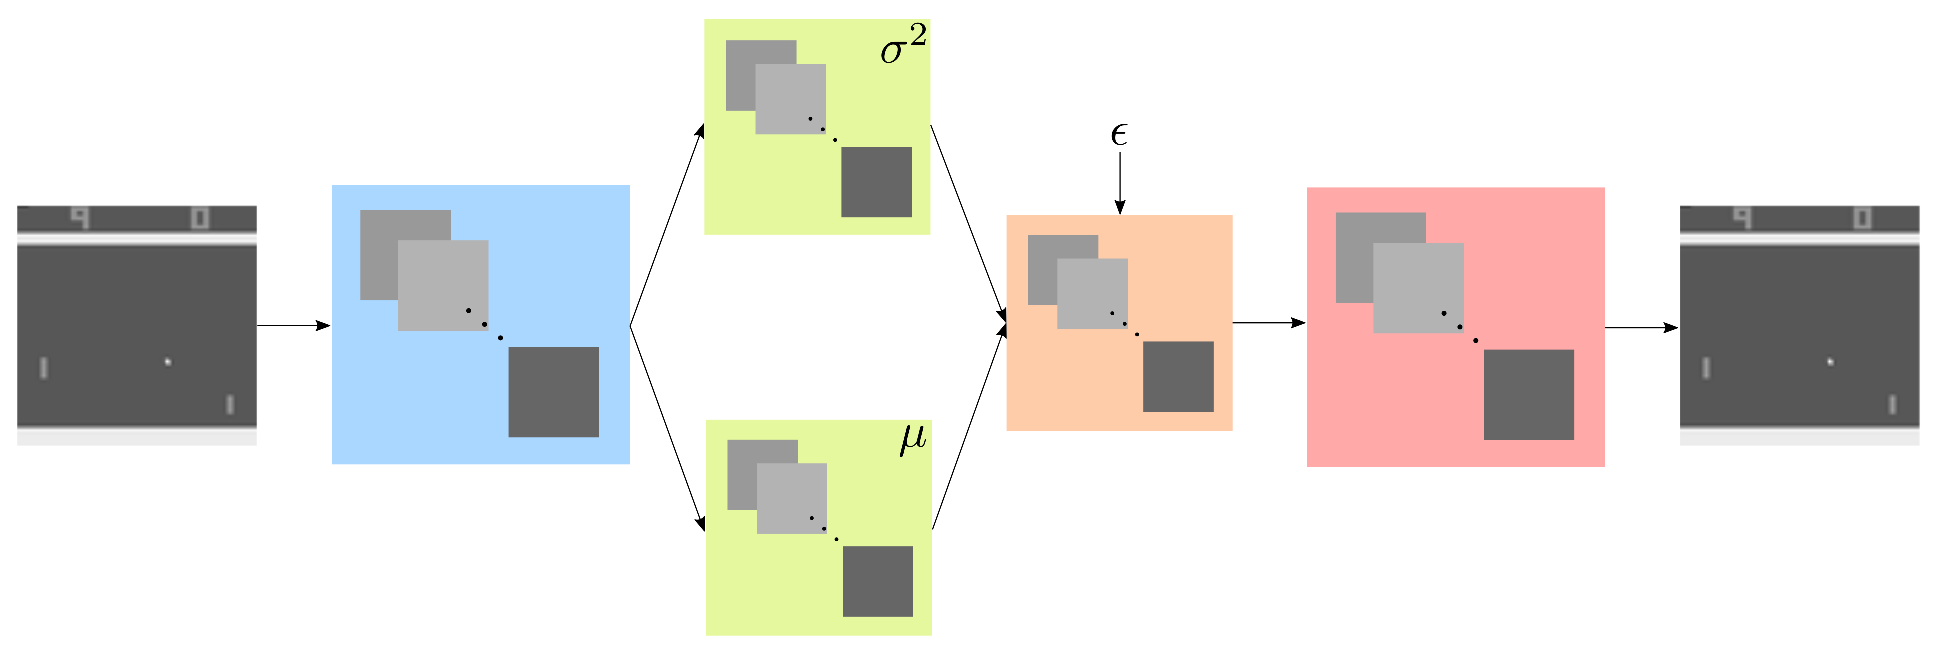
\includegraphics[scale=0.55]{methods/decoupling_indiscriminately_horizontal.eps}
\caption{The fully-convolutional multiple latent filter architecture. \textbf{Blue:} Unchanged. \textbf{Green:} The latent mean $\vec{\mu}$ and variance $\vec{\sigma}^2$, which are both single filters of shape $(k, m, n)$. \textbf{Orange:} A single latent filter of shape $(k, m, n)$ sampled component-wise from $\vec{\mu}$ and $\vec{\sigma}^2$. \textbf{Red:} Unchanged.}
\label{fig:decoupling_indiscriminately_horizontal}
\end{figure}


%
%
\subsection{Constructing a Suitable Loss Function}
\begin{itemize}
\item By the same reasoning for the previous architecture, we keep the reconstruction loss term. 
\item Need to decide on the appropriate term in the loss function to reduce redundancy
\item The latent filter of shape $(k, m, n)$ is flattened to a $k \times m \times n$ vector
\item This flattened representation of the single latent filter is used then pressured to be close to an isotropic Gaussian with KL divergence ...equation here...
\item This pressuring reduces redundancy among all pixels in the latent volume
\end{itemize}

%
%
\subsection{Neuron-Level Decoupling}
\begin{itemize}
\item The latent filter of shape $(k, m, n)$ is flattened to a $k \times m \times n$ vector
\item This flattened representation of the single latent filter is used then pressured to be close to an isotropic Gaussian with KL divergence ...equation here...
\item This pressuring reduces redundancy among all pixels in the latent volume
\end{itemize}

\begin{figure}[H]
\centering
\captionsetup{justification=centering}
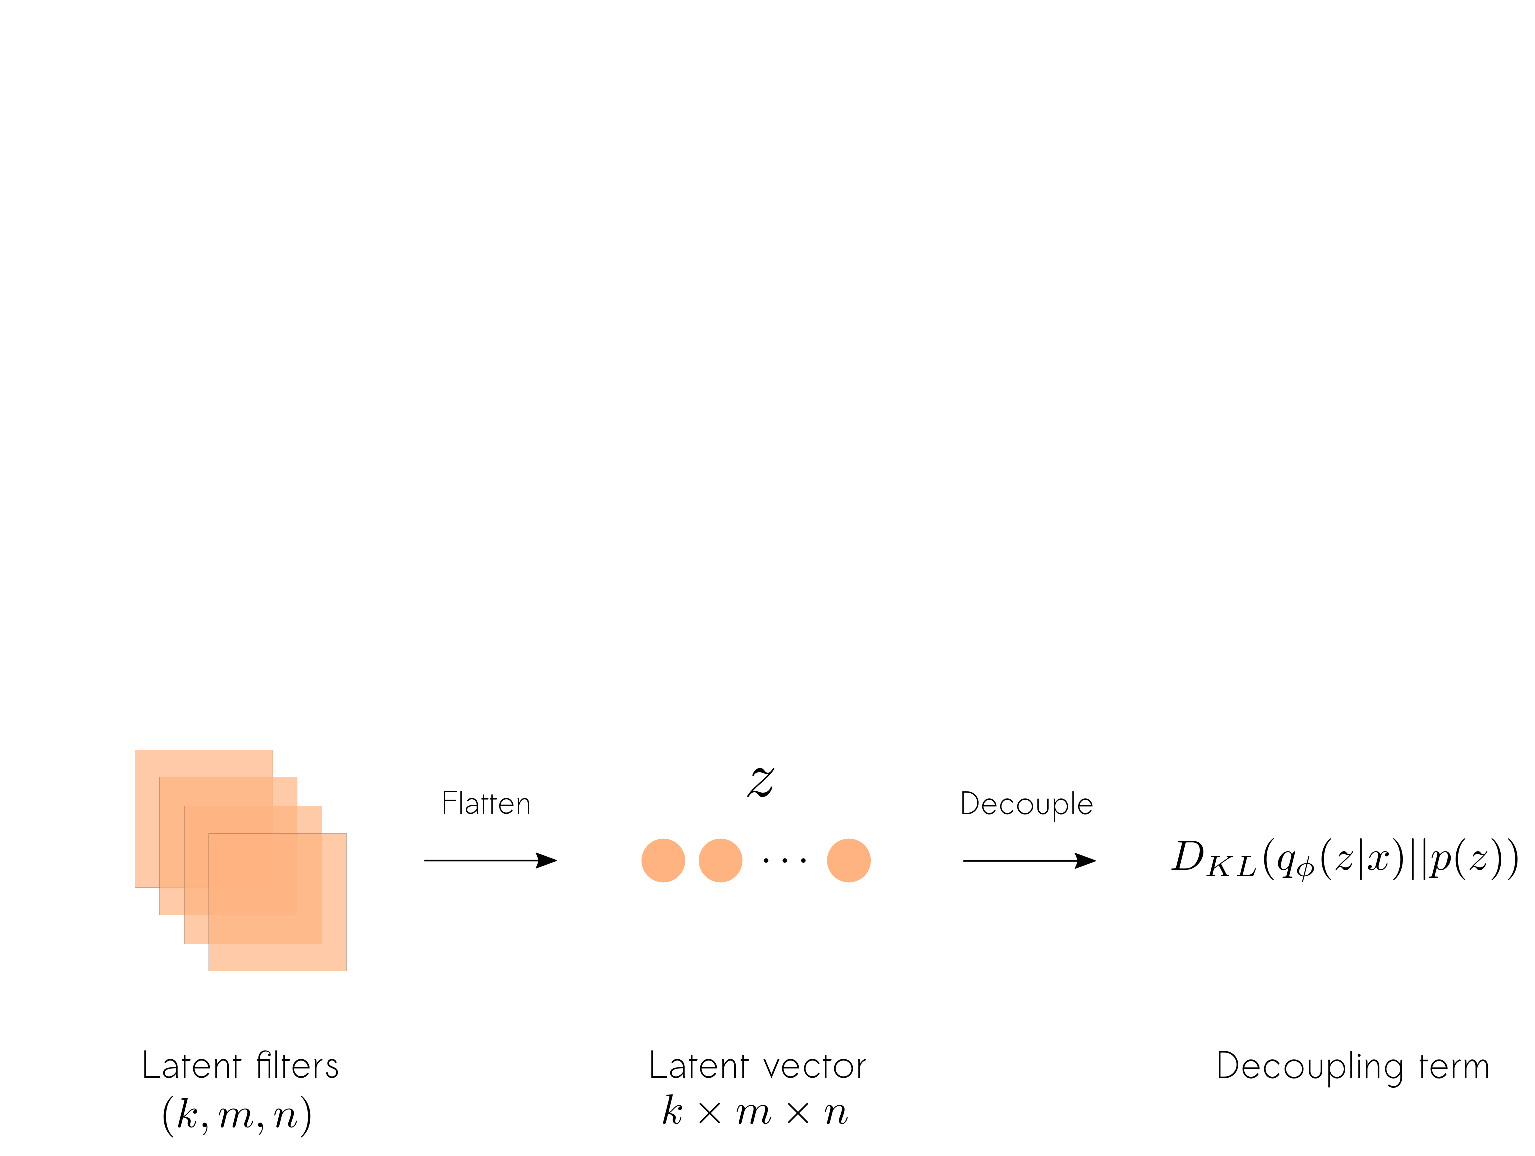
\includegraphics[scale=0.6]{methods/decoupling_indiscriminately_flattening_latent_space.eps}
\caption{Caption.}
\label{fig:decoupling_indiscriminately_flattening_latent_space}
\end{figure}

%
%
\subsection{Na{\"i}ve Filter-Level Decoupling}
\begin{itemize}
\item The $k$ filters of the $(k, m, n)$-dimensional latent space are averaged across their activations and stored in a vector
\item We've reduced our problem to one solved in $\beta$-VAE!
\item To disentangle the average activations over filters, we 
\item This average activation vector of size $k$ is then pressured to be close to an isotropic Gaussian with KL divergence ...equation here...
\item This pressuring reduces redundancy among all pixels in the latent volume
\end{itemize}

\begin{figure}[H]
\centering
\captionsetup{justification=centering}
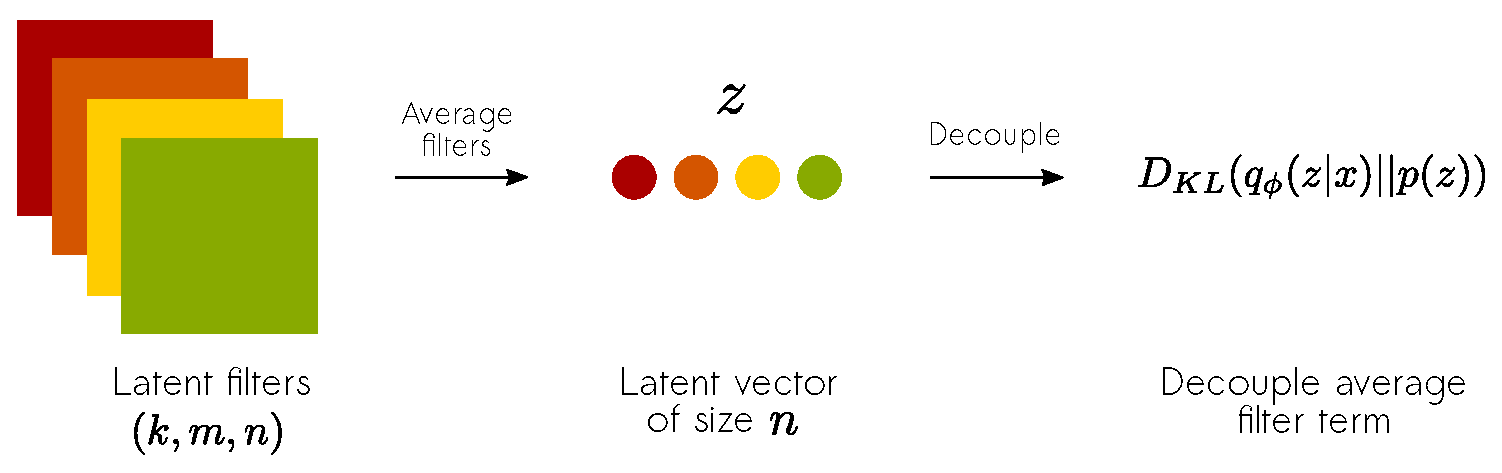
\includegraphics[scale=0.6]{methods/decoupling_averages_latent_space.eps}
\caption{Caption.}
\label{fig:decoupling_averages_latent_space}
\end{figure}

\begin{itemize}
\item The latent filter of shape $(k, m, n)$ is flattened to a $k \times m \times n$ vector
\item This flattened representation of the single latent filter is used then pressured to be close to an isotropic Gaussian with KL divergence ...equation here...
\item This pressuring reduces redundancy among all pixels in the latent volume
\end{itemize}


%
%
\subsection{Weighted Filter-Level Decoupling}
\begin{figure}[H]
\centering
\captionsetup{justification=centering}
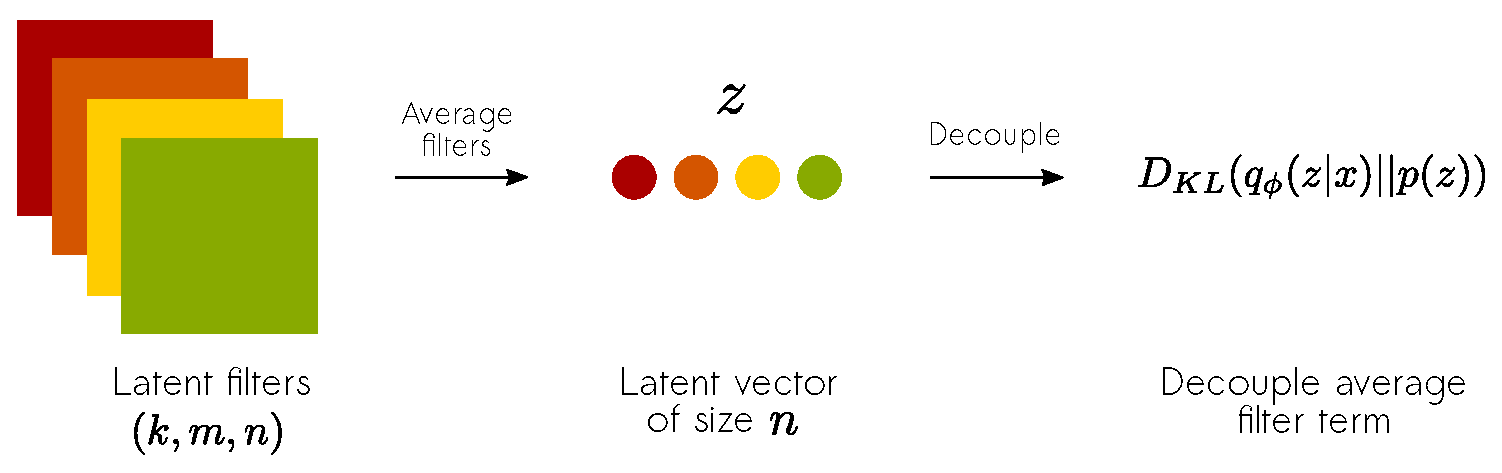
\includegraphics[scale=0.6]{methods/decoupling_averages_latent_space.eps}
\caption{Caption.}
\label{fig:decoupling_averages_latent_space}
\end{figure}



%
%
%
%
%
\section{Separating Colour Spaces}
\subsection{Architecture}
TODO: Finish subsection

\begin{figure}[h!]
\centering
\captionsetup{justification=centering}
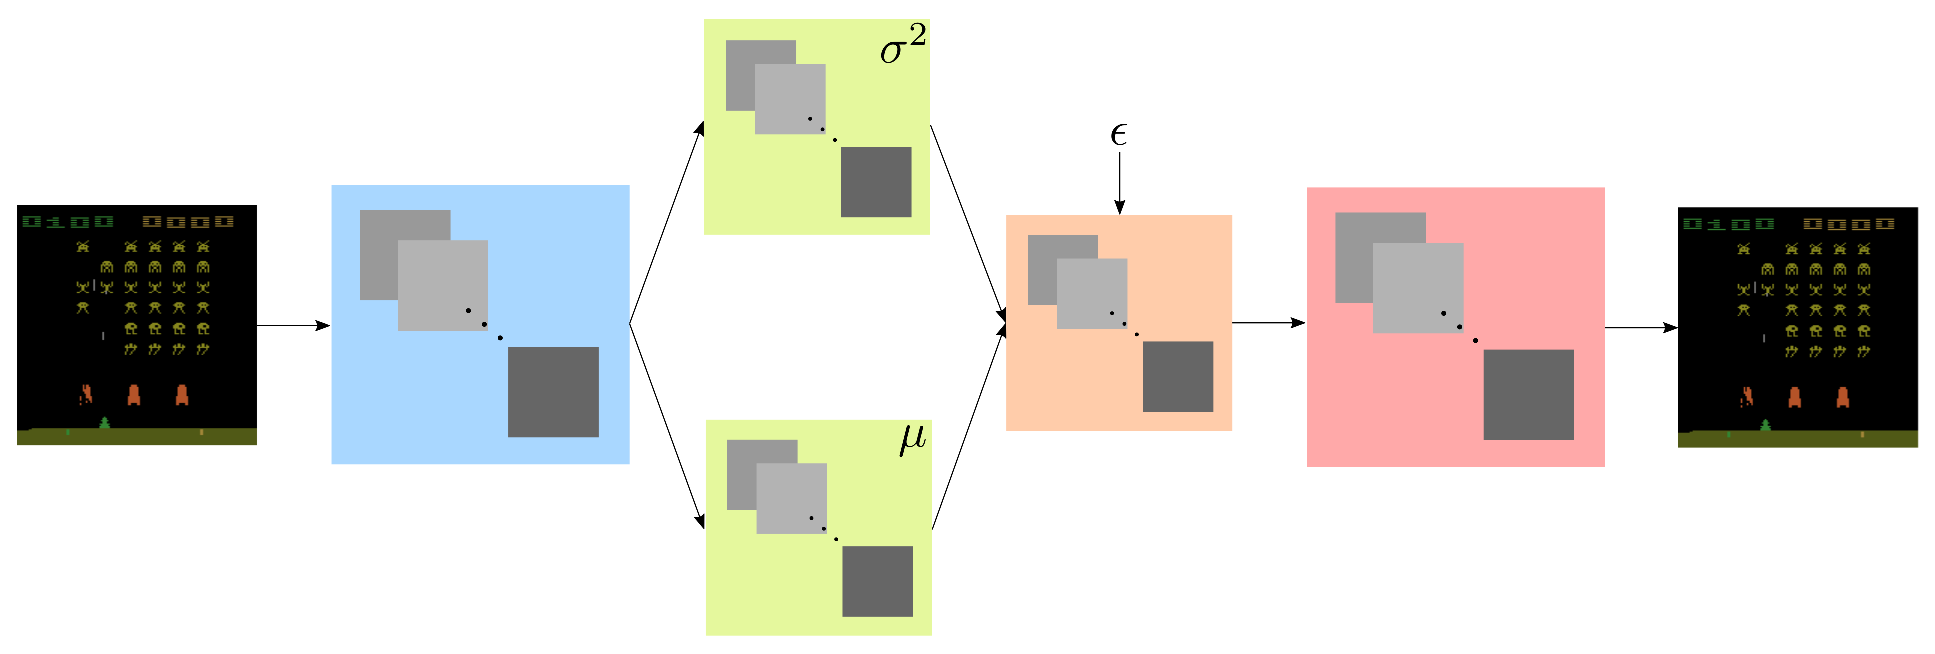
\includegraphics[scale=0.55]{methods/separating_colour_spaces_architecture.eps}
\caption{Caption.}
\label{fig:separating_colour_spaces_architecture}
\end{figure}

\begin{figure*}[h!]
\centering
\captionsetup{justification=centering}
\begin{multicols}{4}
    \includegraphics[scale=0.7]{figures/methods/separating_colour_spaces_original.png}
    \caption{Original}\par
    \includegraphics[scale=0.7]{figures/methods/separating_colour_spaces_r.png}
    \caption{Red}\par
    \includegraphics[scale=0.7]{figures/methods/separating_colour_spaces_g.png}
    \caption{Green}\par
    \includegraphics[scale=0.7]{figures/methods/separating_colour_spaces_b.png}
    \caption{Blue}
\end{multicols}
\caption{A comparison of a $210 \times 160$ RGB frame from Space Invaders and its individual channels. The bullet is clearly separated from other sprites in the blue channel. The barriers TODO: Finish description.}
\label{fig:even_and_odd_frames_space_invaders}
\end{figure*}



\subsection{Derivation}
TODO: Finish subsection

%
%
%
%
%
\section{Orthogonal Convolutions}
\lipsum[2]
\subsection{Architecture}
TODO: Finish subsection
\begin{figure}[h!]
\centering
\captionsetup{justification=centering}
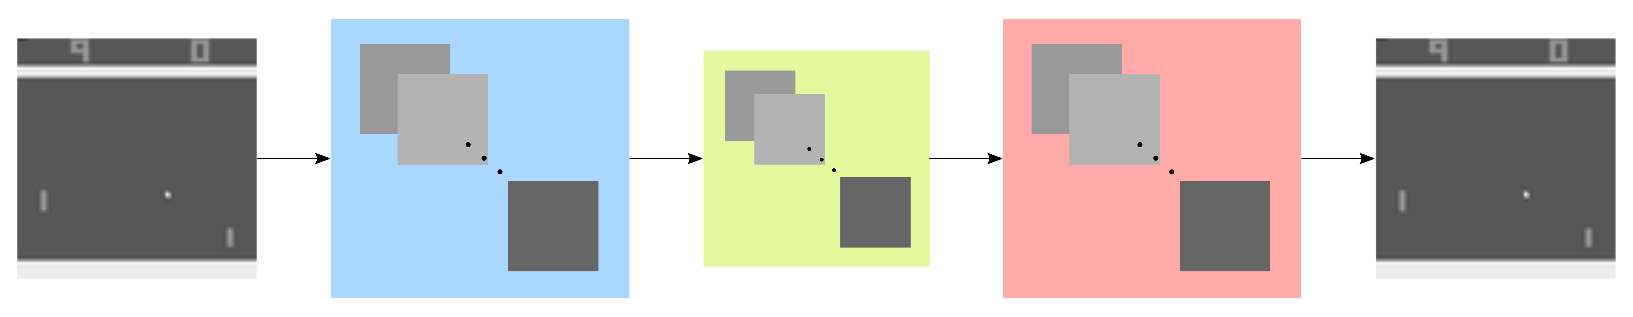
\includegraphics[scale=0.63]{methods/orthogonal_convolutions_archiecture.eps}
\caption{Caption.}
\label{fig:orthogonal_convolutions_archiecture}
\end{figure}

\subsection{Derivation}
TODO: Finish subsection

%
%
%
%
%
\section{Winner Takes All}
\lipsum[2]
\subsection{Architecture}
TODO: Finish subsection
\subsection{Derivation}
TODO: Finish subsection